\documentclass[11pt,a4paper]{article}
\usepackage[T1]{fontenc}
\usepackage[utf8]{inputenc}
\usepackage{lmodern}
\usepackage[margin=25mm]{geometry}
\usepackage{amsmath,amssymb,booktabs,array,graphicx}
\usepackage{microtype}
\usepackage{xcolor}
\usepackage{pgfplots}
\usepgfplotslibrary{groupplots}
\pgfplotsset{compat=1.18}
\usepackage[hidelinks]{hyperref}
\usepackage{xurl}
\setlength{\emergencystretch}{2em}
\newcommand{\method}[1]{\textsf{#1}}
\newcommand{\pending}[1]{\textcolor{red!65!black}{[Author confirmation pending: #1]}}
% Generated from frozen aggregate artifacts. Do not edit.
\newcommand{\RCFone}{0.017292}
\newcommand{\RFone}{0.016603}
\newcommand{\RCRecallPct}{0.8805}
\newcommand{\RCNormalPct}{0.9941}
\newcommand{\RCEpisodes}{554}
\newcommand{\RCEpisodeRate}{185.98}
\newcommand{\FoneGain}{0.000689011}
\newcommand{\ARFone}{0.018846}
\newcommand{\ARAP}{0.507711}
\newcommand{\AREpisodeRate}{437.09}
\newcommand{\TemplateFone}{0.074737}
\newcommand{\TemplateRecallPct}{4.0217}
\newcommand{\TemplateNormalPct}{1.3997}
\newcommand{\PrevalencePct}{50.6268}
\newcommand{\NormalHours}{2.97878}
\newcommand{\FitA}{0.3394252231379215}
\newcommand{\FitB}{0.001855647065541822}
\newcommand{\FitTau}{0.3309050380943476}
\newcommand{\ObserverMSE}{0.338911}
\newcommand{\ARMSE}{0.002094}
\newcommand{\AmbiguityPct}{53.12}

\title{Correction Evidence in Robotic Motion Monitoring:\\A Controlled CASPER Study}
\author{Muhammad Usman \and Haiqa Mushtaq}
\date{Working draft --- 17 October 2026}
\begin{document}
\maketitle
\noindent\textbf{Draft status.} Author names follow the order supplied for this project. Affiliations, contribution roles, funding, conflicts and approval by both authors remain unconfirmed. This local draft has not been submitted, externally reviewed or PDF-validated.
\begin{abstract}
% claim: AB01
Does the evidence in a motion observer's measurement correction improve anomaly detection beyond its prospective residual? We examine this question on one original CASPER right-arm recording containing eight scheduled speed-intervention intervals. An empirical categorical phase observer predicts twelve joint-position and joint-velocity measurements from a fixed periodic reference. The primary comparison adds a training-scaled Jensen--Shannon correction discrepancy while preserving the same observer state trajectory. Eleven deterministic score and control variants are fitted or specified using normal data, frozen before threshold-only calibration, and evaluated through continuous protected replay. All methods produce 897,119 finite eligible scores. Adding correction evidence increases unadjusted F1 from \RFone\ to \RCFone\ and slightly reduces normal alarm burden. Nevertheless, positive-point recall is only \RCRecallPct\%, with \RCEpisodeRate\ normal alarm episodes per eligible hour. Fresh alarms occur in all eight intervention intervals, showing why event hits must be interpreted alongside sparse point coverage and frequent normal alarms. An ordinary autoregression achieves higher F1 and average precision with more alarm episodes; a fixed periodic template attains the largest F1 with higher point false alarms. The result is a small within-recording correction-score effect, not evidence of a generally effective detector. Both primary variants retain progression, and no validated physical digital twin or cross-robot generalization is established. The accompanying local package preserves the complete comparison, source identities and deterministic table/figure generation; broader confirmation requires fresh independent evidence.
\end{abstract}

\noindent\textbf{Keywords:} robotic motion monitoring; anomaly detection; phase observer; correction evidence; CASPER; evaluation methodology.
\section{Introduction}
\label{sec:intro}
% claim: I01
A motion monitor for a repetitive robot must account for where the robot is in its task. The same joint position can be expected at one stage and inconsistent with another. Existing robot-monitoring studies use temporal alignment, prediction or execution progress to make this distinction: CASPER evaluates motion anomalies using external inertial measurements, while progress-dependent monitoring and Bayesian interaction primitives explicitly represent temporal state~\cite{casper2024,park2016,campbell2017}. These precedents motivate a precise question about an observer's output: does the evidence contained in a measurement correction improve detection beyond its prospective prediction error?

% claim: I02
Prediction and correction serve different purposes. A predictor estimates the next observation from available history. A measurement update then changes the state estimate to account for the new observation. Innovation-based failure detection and the relationship between tracking sensitivity and residuals are established topics~\cite{willsky1976}. Likewise, posterior-to-prior divergence is an established measure of Bayesian surprise~\cite{itti2005}. Their existence does not imply that combining a residual with a correction statistic will improve a particular security monitor. A normal observation can legitimately change a phase estimate, and an abnormal observation can be poorly explained without greatly redistributing phase weights.

% claim: I03
We examine that question on the original CASPER right-arm recording using joint positions, joint velocities and relative elapsed time. A fixed empirical phase observer supplies a prospective residual and a Jensen--Shannon correction discrepancy. The primary comparison adds the discrepancy to the residual while holding the observer trajectory, observations, fitted reference and evaluation support constant. Both variants already incorporate nominal progression. This comparison therefore isolates an added score term, not the presence of progression or a new state estimator.

% claim: I04
The study provides three bounded outputs: an explicit same-observer comparison with classical surprise and ordinary controls; a complete chronological evaluation that separates normal calibration from final outcomes; and a reproducible record of the resulting detection--false-alarm trade-offs. All eleven deterministic methods are retained. The scope is a descriptive study of one acquisition, not a claim that phase estimation or score fusion is new, nor a reproduction of published CASPER performance. We use the term \emph{empirical motion observer}: the implementation has measured-state correspondence and causal synchronization, but no validated robot dynamics or independently calibrated physical-state uncertainty.

% claim: I05
The findings support only a small correction-score effect. Absolute detection is weak, and simple controls match or exceed several observer outcomes. Reporting this result requires more than counting event hits. A detector that alarms often during normal motion can intersect every long intervention interval while recognizing few of its positive observations. We therefore examine point metrics, alarm episodes, complete event outcomes and schedule-relative delays together. This choice follows the broader need to align security-learning evaluation with the information and operational setting being claimed~\cite{arp2022}.

\section{Related work and comparison scope}
\label{sec:related}
% claim: W01
\paragraph{Robot monitoring and digital-twin frameworks.}
CASPER uses an external inertial measurement unit (IMU), periodic/statistical references and learned next-observation predictors to detect altered arm motion~\cite{casper2024}. Its later edge-computing study combines task segmentation with prediction on external IMU signals~\cite{edge2025}. Our controller-input experiment changes the observation and trust boundary. Consequently, published scores from those experiments are not entries in our numerical comparison, and our implementations are not called CASPER reproductions.

% claim: W02
TWINE describes a digital-twin and explainable-learning framework using a supervised random-forest classifier. Its accepted manuscript specifies an 80/20 train--test split using \texttt{train\_test\_split} and labelled training examples~\cite{twine2026}. Our fit and model-selection partitions contain normal observations only and are chronological. Moving TWINE into this task would change its supervision and input protocol; retaining attack-labelled training would instead change ours. We therefore treat it as related framework work rather than an admitted normal-only comparator. We do not reproduce its cloud deployment or make a standards-compliance claim for our observer.

% claim: W03
\paragraph{Phase, alignment and prospective prediction.}
Bayesian Interaction Primitives jointly infer phase, phase velocity and trajectory state~\cite{campbell2017}. Periodic Interaction Primitives address repeated motion through periodic representations and observation-conditioned inference~\cite{clark2020}. Park et al. use a hidden Markov model (HMM) with a distribution over execution progress and a progress-dependent anomaly threshold~\cite{park2016}. These works establish that phase-aware monitoring and state correction are not new by themselves. Their platforms, modalities and tasks differ from the present recording. We neither import their reported performance nor claim superiority over implementations that were not run.

% claim: W04
\paragraph{Residual and distributional evidence.}
Classical innovation monitoring separates prediction error from state correction~\cite{willsky1976}. Bayesian surprise measures posterior-to-prior Kullback--Leibler (KL) divergence~\cite{itti2005}. Anomaly Transformer combines reconstruction error with a discrepancy between attention associations~\cite{xu2022}; those associations are not our phase probabilities. These precedents motivate retaining KL surprise and predictive mixture energy alongside the chosen Jensen--Shannon statistic. They also preclude a generic novelty claim based on combining error and discrepancy.

% claim: W05
Our comparison set is defined by the narrow scientific question. It contains a matched residual/correction pair, explanatory scores from the same observer, two state-update variants and three ordinary controls. It does not establish competitive performance against the full recent neural-detection literature. The project's recent-paper screen covered 16 October 2023 through 16 October 2026; older references here are methodological foundations, not recent experimental baselines. Source versions, manuscript-access gaps and paper-to-code decisions are recorded in the accompanying reference and comparator registers.

\section{Problem, threat model and data}
\label{sec:data}
% claim: D01
\subsection{Observation and trust boundary}
At observation index $t$, the monitor receives six actual joint positions $q_t$, six actual joint velocities $\dot q_t$, and elapsed native time $\Delta t$. Positions and velocities are interpreted in radians and radians per second, respectively, following the audited controller-field mapping. The model cannot use labels, source-row identifiers, absolute clock values, commanded targets, safety status, current, torque, other-arm channels, network traffic or external IMU measurements. Source coordinates remain available to the evaluator for alignment. The velocity control intentionally uses only the six-velocity subset of the shared information budget.

% claim: D02
The restricted adversary alters the command/application path governing motion speed while the monitoring telemetry and its clock remain truthful. The dataset does not establish authenticated telemetry or resistance to compromised controller firmware. The study asks whether scheduled speed interventions produce detectable deviations under this assumption. It does not identify the adversary's entry point, infer malicious intent, distinguish faults from authorized changes, or demonstrate mitigation. If authorized and unauthorized actions produce identical permitted observation histories, a detector using only those histories cannot distinguish them. That is an input-identifiability limit, not an empirical failure rate estimated here.

% claim: D03
\subsection{Release identity and annotation meaning}
We use the original CASPER provider collection, version 3, rather than the separate later ``CASPER 1 \& 2'' listing~\cite{casperdata}. The selected original file is \texttt{dataset/right\_arm.csv}, containing 1,762,650 data rows. Its byte size is 1,978,193,094 and its SHA-256 identity is given in Appendix~\ref{app:identity}. The file was retained unchanged. Our right-arm route is distinct from the externally sensed detection experiment described in the CASPER paper~\cite{casper2024}.

% claim: D04
Local schema and annotation audits established twelve selected joint-state channels, native controller timing and eight contiguous positive flag intervals. The flags describe a scheduled intervention program. They are not independently measured physical-impact onsets, and a zero flag after an intervention is not proof of complete physical recovery. Matched capture-source inspection indicates that the same flag was written to both arm logs while the right-arm speed changed; the left arm therefore does not supply a second independent attacked robot. Cross-device synchronization with the IMU or packet trace was not established and is unnecessary for this single-stream analysis.

% claim: D05
This is one repetitive pick-and-place acquisition. The eight scheduled intervals, millions of samples and repeated motion cycles are dependent observations from that acquisition. The dataset provides no independent labels for legitimate changeovers, attack intent or corresponding mechanical faults within our admitted track. We retain these limitations when interpreting every detection count. No other dataset or synthetic attack was added to the final comparison.

\section{Empirical observer and comparison methods}
\label{sec:methods}
% claim: M01
\subsection{Training-only reference and scaling}
Let $x_t=(q_t,\dot q_t)\in\mathbb R^{12}$. Training-only population moments give
\begin{equation}
 z_{t,j}=\frac{x_{t,j}-\mu_j}{\sigma_j},\qquad
 \sigma_j^2=\frac{1}{n_{\rm fit}}\sum_{t\in\mathcal T}(x_{t,j}-\mu_j)^2.
 \label{eq:scale}
\end{equation}
Moments are accumulated using Welford's algorithm. Constant or nonfinite channels fail admission; no clipping, imputation, resampling or future-looking interpolation is used. All reference/parameter fitting uses the 536,946 eligible training targets. Warmup observations can initialize causal state but are excluded from those fitting targets.

% claim: M02
The periodic reference comprises $B=32$ standardized mean vectors $m_k$ and a training-estimated period $T=38$ seconds. Period estimation samples every twentieth observation from the first eligible training segment, up to 10,000 observations. It examines mean squared twelve-channel differences for lags 1--121; candidates 2--120 must be local minima. Minimum objective, then smaller lag, breaks ties. The selected lag is converted using actual elapsed-time differences. For each candidate bin count, a bootstrap clock template initializes a fixed phase offset from each segment's warmup, after which eligible training endpoints produce the final bin means. Empty bins or missing admissible periods fail. Appendix~\ref{app:selection} records the finite configuration search; no final outcome selected the period or bins.

% claim: M03
\subsection{Phase propagation and measurement correction}
The dynamic state is a categorical distribution over the $B$ phase bins. Each segment begins uniformly. Given previous posterior $p^+_{t-1}$ and native $\Delta t$, define the circular shift operator $\mathcal S_\delta$ by linearly distributing probability between adjacent bins for a forward displacement $\delta=B\Delta t/T$. The prior is
\begin{equation}
 p^-_t=(1-\epsilon_t)\mathcal S_{B\Delta t/T}p^+_{t-1}
       +\epsilon_t\frac{\mathbf 1}{B},\quad
 \epsilon_t=1-\exp(-0.02\Delta t).
 \label{eq:prior}
\end{equation}
This is a fixed empirical transition, not an identified robot-dynamics equation. Repeated fractional shifts introduce numerical diffusion.

% claim: M04
Before the current measurement influences state, the observer predicts
\begin{equation}
 \widehat z_t=\sum_{k=0}^{B-1}p^-_t(k)m_k,\qquad
 R_t=\frac{1}{12}\|z_t-\widehat z_t\|_2^2.
 \label{eq:residual}
\end{equation}
The current observation then supplies template distances and a tentative posterior:
\begin{align}
 D_t(k)&=\frac{1}{12}\|z_t-m_k\|_2^2,\quad e_t(k)=\frac{D_t(k)}{2\tau},\\
 Z_t&=\sum_k p^-_t(k)\exp[-e_t(k)],\quad
 p^+_t(k)=\frac{p^-_t(k)\exp[-e_t(k)]}{Z_t}.
 \label{eq:posterior}
\end{align}
Normalization is computed stably in log space. The bandwidth is the larger of $10^{-8}$ and the training mean of $\min_k D_t(k)$; its fitted value is $\tau=\FitTau$. These radial-basis weights are a pseudo-likelihood, not a calibrated model of physical sensor noise.

% claim: M05
With $u_t=(p^-_t+p^+_t)/2$, correction evidence is
\begin{equation}
 C_t=\tfrac12\mathrm{KL}(p^-_t\|u_t)+\tfrac12\mathrm{KL}(p^+_t\|u_t).
 \label{eq:js}
\end{equation}
Natural logarithms are used; zero-mass terms contribute zero. The statistic lies in $[0,\log 2]$ apart from numerical tolerance. It measures unsigned belief redistribution, not physical phase error, speed or attack probability. All scores are emitted before the tentative posterior is committed. No score changes the fitted reference, bandwidth, normalizer or threshold.

% claim: M06
\subsection{Primary contrast and explanatory scores}
Training-only mean residual and correction values are $a=\FitA$ and $b=\FitB$. The primary scores are
\begin{equation}
 S_{\mathrm{O-R},t}=R_t/a,\qquad
 S_{\mathrm{O-RC},t}=R_t/a+C_t/b.
 \label{eq:primary}
\end{equation}
Both scores use exactly the same prior, posterior, prediction and subsequent state trajectory. Removing $C_t/b$ does not remove progression or measurement correction from the observer. The sum has equal coefficients after training-mean scaling; no fusion-weight search was performed.

% claim: M07
Four explanatory outputs use that same observer: \method{O-C} is raw $C_t$; \method{O-K} is $\mathrm{KL}(p^+_t\|p^-_t)$; \method{O-L} is the predictive mixture energy $-\log Z_t$; and \method{O-Rv} is the mean standardized squared residual restricted to the six velocity channels. The last output still obtains its state from all twelve channels. Two auxiliary update policies retain $R_t/a$: \method{O-Follow} uses likelihood-only phase correction after warmup, while \method{O-Free} omits measurement correction after warmup but keeps nominal propagation and mixing. All three policies share ordinary correction during initialization. The free-running distribution's diffusion limits what this comparison says about fixed references.

% claim: M08
The energy and KL outputs are related by the direct identity
\begin{equation}
 -\log Z_t=\mathrm{KL}(p^+_t\|p^-_t)+\sum_k p^+_t(k)e_t(k),
 \label{eq:energyidentity}
\end{equation}
for positive prior support. Also,
\begin{equation}
 \sum_k p^-_t(k)D_t(k)=R_t+
 \frac1{12}\sum_k p^-_t(k)\|m_k-\widehat z_t\|_2^2.
 \label{eq:mixtureidentity}
\end{equation}
These algebraic decompositions motivate conventional controls and ambiguity analysis; they are not claimed as new theorems. Jensen--Shannon discrepancy has no identical KL decomposition. Equally poor likelihoods can leave a posterior unchanged, whereas an informative normal measurement can change it substantially.

% claim: M09
\subsection{Ordinary controls}
\method{V-Z} takes the maximum absolute training-standardized deviation across joint velocities. \method{T-32} predicts from the fixed 32-bin template. Its warmup chooses the minimum cumulative-loss integer phase offset, with the smallest offset breaking ties; thereafter only elapsed time advances the phase. It makes no current-observation phase adjustment.

\method{AR-4} is a separate autoregression for each standardized channel,
\begin{equation}
 \widehat z_{t,j}=\alpha_j+\sum_{\ell=1}^{4}\beta_{j,\ell}z_{t-\ell,j}.
 \label{eq:ar}
\end{equation}
Training minimizes mean squared prediction error plus $0.001\sum_\ell\beta_{j,\ell}^2$, with an unpenalized intercept. Its score is mean twelve-channel squared residual. The current sample enters history only after scoring. This is teacher-forced one-step monitoring, not autonomous simulation or a cross-channel vector autoregression. Singular/nonfinite fits fail rather than trigger altered regularization. These controls are our implementations; none is a claimed faithful reproduction of a cited paper.

\section{Evaluation design and execution}
\label{sec:evaluation}
% claim: E01
\subsection{Chronological partitions and common support}
Table~\ref{tab:splits} defines zero-based data rows excluding the header, with half-open ranges. Splitting precedes history construction. A new segment begins when $\Delta t\leq0$ or $\Delta t>0.075$ seconds. Each partition starts independently, except that final normal and mixed slices are two reporting regions of one continuous replay. Every method excludes the same first 1,528 observations after a segment start; no method-specific denominator is trimmed. Training contains a restart at row 16,571. Final replay contains one initial warmup and no later resets.

\begin{table}[htbp]\centering\small
\caption{Frozen populations. The mixed slice continues the final-normal state.}\label{tab:splits}
\begin{tabular}{lrrr}\toprule
Purpose & Raw rows $[a,b)$ & Raw count & Eligible count\\\midrule
Training & $[0,540002)$ & 540,002 & 536,946\\
Normal development & $[540002,702002)$ & 162,000 & 160,472\\
Normal calibration & $[702002,864003)$ & 162,001 & 160,473\\
Protected normal & $[864003,1080004)$ & 216,001 & 214,473\\
Protected mixed & $[1080004,1762650)$ & 682,646 & 682,646\\\bottomrule
\end{tabular}\end{table}

% claim: E02
\subsection{Selection, freezing and threshold calibration}
Seven ordinary candidates were declared: one velocity control, two templates with 32/64 bins, and four autoregressions crossing orders 1/4 with ridge values 0.001/0.1. Template and autoregression selection separately minimized normal-development prediction mean squared error (MSE), with declared candidate order resolving ties. No cross-family winner was selected. The 32-bin template and order-4, ridge-0.001 autoregression were retained without refitting on development. The observer reused the selected template and the same normal development for internal checks; this reuse is disclosed rather than described as independent validation. Its mixing rate and scoring definitions had no outcome-driven sweep.

% claim: E03
The complete eleven-method roster, fitted artifacts, transformations, initialization, formulas, budgets and reporting rules were locally frozen before calibration. These records are prospective experiment records, not an externally registered study or independently blinded protocol. Each method then received the same 160,473 eligible normal-calibration scores. For ascending scores $s_{(i)}$, the fixed operating point is
\begin{equation}
 \theta=s_{(158869)},\qquad A_t=\mathbf 1[S_t>\theta],
 \label{eq:threshold}
\end{equation}
where $158869=\lceil0.99\times160473\rceil$. Strict exceedance handles ties. Calibration sets thresholds only; it cannot choose a model, seed, combination, percentile, persistence rule or checkpoint. This empirical quantile does not guarantee a future 1\% false-alarm rate.

% claim: E04
\subsection{Outcome definitions}
The mixed population contains 345,602 schedule-positive and 337,044 schedule-zero observations. Unadjusted precision, recall and F1 use counts of true positives (TP), false positives (FP), false negatives (FN) and true negatives (TN). Average precision (AP) groups equal scores, evaluates precision after each whole tie group enters, and sums precision times recall increments. There is no point adjustment or test-optimized threshold. Undefined quantities are retained as undefined rather than replaced by a favorable number. Mixed prevalence is reported because it affects precision and the constant-score AP reference.

% claim: E05
Protected-normal burden comprises the fraction of eligible points alarmed and the number of contiguous alarm episodes per eligible native-time hour. Exposure sums adjacent eligible timestamp differences within a continuous segment; it does not substitute a nominal sample count for elapsed time. Episodes crossing report boundaries or warmup are explicitly classified. Schedule-zero mixed intervals are reported separately from the held-out normal population and are not assumed to be certified recovery.

% claim: E06
An event-overlap hit requires an alarm on at least one eligible positive point. A fresh onset requires the start of a new alarm episode within the interval; an alarm already active at the boundary can overlap without being fresh. Delay is measured from the recorded flag onset to the first qualifying alarm. Misses retain null delays and remain in the eight-event denominator. Detected-only summaries explicitly state the number detected. No attack boundary initializes phase or changes a score, threshold or state. There is no cooldown or persistence filter.

% claim: E07
\subsection{Protected execution and integrity checks}
All eleven methods are deterministic and ran once, with no stochastic seed. The policy seeds 17, 42 and 2026 were reserved for stochastic methods; none was admitted. Final feature replay saved all aligned scores and hashes without parsing labels. The delayed evaluator was admitted only after the complete score seal and accepted resource-supervisor receipt. Joint outcomes were inspected after every evaluation completed. One scoring attempt and one evaluation attempt succeeded; there were no failed final attempts or retries.

% claim: E08
The implementation was covered by 324 synthetic software tests. The same 52 source/configuration identities and 133 frozen input bindings remained unchanged during the campaign. A separate saved-result audit recomputed metric, episode, event and recovery arithmetic, with seven hand-checkable synthetic examples preceding it. Its millions of coordinate assertions are software checks, not independent experiments. It did not reopen raw observations or replay a detector. Original-label verification belonged to the evaluator; the supplemental arithmetic audit reconstructed labels from the frozen schedule and was not independent reannotation.

\section{Results}
\label{sec:results}
% claim: R01
\subsection{Coverage and normal-development correspondence}
Every method produced 897,119 finite eligible final scores: 214,473 in the protected normal slice and 682,646 in the mixed slice. Eligible coverage is 100\%. Raw final coverage is 99.829967\%; the only 1,528 exclusions are the common initial warmup. No missing scores explain the weak detection. Protected-normal exposure is \NormalHours\ hours for every method.

% claim: R02
Earlier normal-only checks supported a recurring 38-second reference and prospective state synchronization, but did not establish accurate latent phase. The synchronized observer's development one-step MSE was \ObserverMSE, compared with \ARMSE\ for the ordinary autoregression. The declared ambiguity criterion was met at \AmbiguityPct\% of sampled diagnostic endpoints. The criterion used normalized entropy above 0.5 or circular resultant below 0.5; these are descriptive diagnostics, not calibrated confidence bounds or independently observed phase errors. This evidence already limited the observer interpretation before final scoring.

% claim: R03
\subsection{Point detection and normal alarm burden}
Table~\ref{tab:results} shows all declared methods in their frozen order. \method{O-RC} achieved F1 \RCFone\ and point recall \RCRecallPct\%. Its protected-normal point alarm fraction was \RCNormalPct\%, with \RCEpisodes\ episodes or \RCEpisodeRate\ episodes per eligible hour. Thus a point-alarm fraction close to the calibration percentile coexisted with frequent alarm episodes. No method exceeded \TemplateRecallPct\% point recall.

\begin{table}[htbp]\centering\scriptsize
\caption{Complete final comparison. Precision, recall, F1 and AP are fractions. Normal point alarms are percentages; episodes/h uses eligible protected-normal exposure. Hits are event overlaps out of eight. No scores are point-adjusted.}\label{tab:results}
\resizebox{\textwidth}{!}{\begin{tabular}{lrrrrrrr}
\toprule
Method & Precision & Recall & F1 & AP & Normal (\%) & Episodes/h & Hits \\
\midrule
O-R & 0.465869 & 0.008452 & 0.016603 & 0.506108 & 1.0067 & 189.34 & 7/8 \\
O-RC & 0.478459 & 0.008805 & 0.017292 & 0.506414 & 0.9941 & 185.98 & 8/8 \\
O-C & 0.509185 & 0.009705 & 0.019047 & 0.506135 & 0.9861 & 342.76 & 8/8 \\
O-K & 0.505838 & 0.009777 & 0.019183 & 0.506193 & 0.9917 & 349.47 & 8/8 \\
O-L & 0.465875 & 0.008513 & 0.016720 & 0.506284 & 1.0053 & 189.34 & 7/8 \\
O-Rv & 0.465476 & 0.008446 & 0.016591 & 0.502845 & 1.0048 & 189.34 & 7/8 \\
O-Follow & 0.465551 & 0.008368 & 0.016441 & 0.504844 & 1.0043 & 189.34 & 7/8 \\
O-Free & 0.466422 & 0.008461 & 0.016620 & 0.506295 & 0.9964 & 189.34 & 7/8 \\
V-Z & 0.462248 & 0.008414 & 0.016528 & 0.506759 & 0.9969 & 189.34 & 7/8 \\
T-32 & 0.527677 & 0.040217 & 0.074737 & 0.490596 & 1.3997 & 200.42 & 8/8 \\
AR-4 & 0.500603 & 0.009604 & 0.018846 & 0.507711 & 0.9833 & 437.09 & 8/8 \\
\bottomrule
\end{tabular}
}
\end{table}

\begin{figure}[htbp]\centering
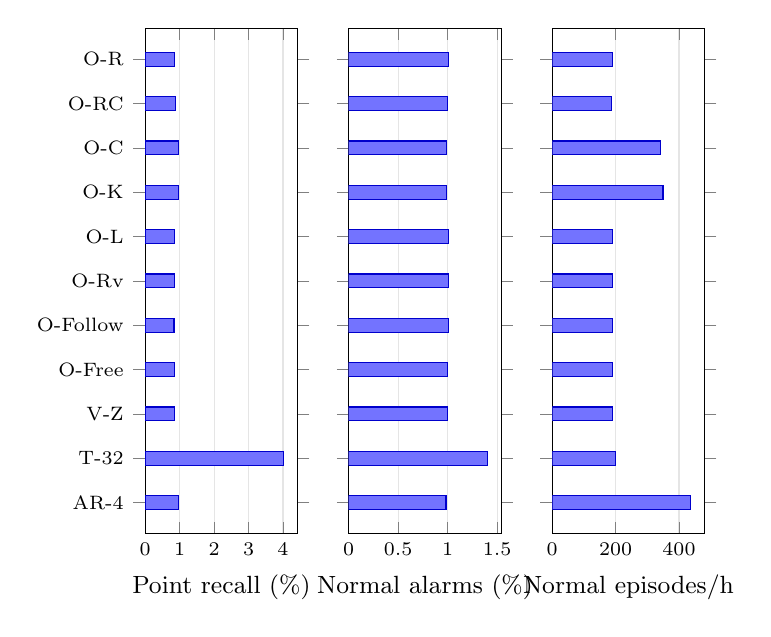
\begin{tikzpicture}
\begin{groupplot}[group style={group size=3 by 1,horizontal sep=0.65cm},width=0.29\textwidth,height=8cm,xbar,/pgf/bar width=5pt,ymin=-0.7,ymax=10.7,ytick={0,...,10},yticklabels={O-R,O-RC,O-C,O-K,O-L,O-Rv,O-Follow,O-Free,V-Z,T-32,AR-4},y dir=reverse,xmin=0,tick label style={font=\scriptsize},label style={font=\small},xmajorgrids=true,grid style={gray!20}]
\nextgroupplot[xlabel={Point recall (\%)}]
\addplot[fill=blue!55,draw=blue!80!black] coordinates {(0.8451918681,0) (0.8804925897,1) (0.9704804949,2) (0.9777142493,3) (0.8512682218,4) (0.8446131677,5) (0.836800713,6) (0.8460599186,7) (0.8414303158,8) (4.021678115,9) (0.9603532387,10)};
\nextgroupplot[xlabel={Normal alarms (\%)},yticklabels={}]
\addplot[fill=blue!55,draw=blue!80!black] coordinates {(1.006653518,0) (0.9940645209,1) (0.9861381153,2) (0.9917332252,3) (1.005254741,4) (1.004788482,5) (1.004322222,6) (0.9963958167,7) (0.9968620759,8) (1.399709987,9) (0.9833405604,10)};
\nextgroupplot[xlabel={Normal episodes/h},yticklabels={}]
\addplot[fill=blue!55,draw=blue!80!black] coordinates {(189.3394009,0) (185.9823194,1) (342.758029,2) (349.4721922,3) (189.3394009,4) (189.3394009,5) (189.3394009,6) (189.3394009,7) (189.3394009,8) (200.4177702,9) (437.0920213,10)};
\end{groupplot}
\end{tikzpicture}

\caption{Detection and false-alarm burden for every declared method. Axes use different units as labelled; bars start at zero. This descriptive figure has no independent-acquisition uncertainty intervals. Values are generated from the saved final summary.}\label{fig:tradeoffs}
\end{figure}

% claim: R04
The primary \method{O-RC} minus \method{O-R} contrast increased F1 by \FoneGain. It added 122 true-positive points while removing 32 mixed false-positive points, 27 protected-normal alarm points and ten protected-normal episodes. Normal episode rate decreased by 3.3571/hour. These paired recorded outcomes are slightly favorable to the added correction term, with unchanged coverage. Their small size and low absolute recall do not establish useful general detection or a newly effective security mechanism.

% claim: R05
The ordinary \method{AR-4} achieved F1 \ARFone\ and AP \ARAP, both above \method{O-RC}, with slightly fewer normal alarm points (2,109 versus 2,132). It produced 1,302 normal episodes, or \AREpisodeRate/hour, compared with 554 for \method{O-RC}. The fixed template \method{T-32} achieved the largest F1 (\TemplateFone) and recall (\TemplateRecallPct\%), but its normal point alarms reached \TemplateNormalPct\% and mixed scheduled-zero alarms 3.6912\%. These are trade-offs, not a single global ranking. No scalar utility was declared to choose a winner after exposure.

% claim: R06
Mixed positive prevalence was \PrevalencePct\%. The constant tied-score AP reference is that prevalence; observed AP ranged from 0.490596 to 0.507711. Values near this reference do not establish useful broad ranking separation. This reference is arithmetic, not an additional detector run. Precision reflects the recorded schedule's unusually high positive prevalence and is not an estimated field attack precision.

% claim: R07
\subsection{Explanatory scores and update-policy ablations}
Correction-only \method{O-C} and KL surprise \method{O-K} had slightly higher F1 than \method{O-RC}, but 342.76 and 349.47 normal episodes/hour, respectively. The energy score \method{O-L}, velocity residual \method{O-Rv}, free-running and unconstrained-following residuals remained close to \method{O-R} on the reported point outcomes. The direct velocity control was also similar. These are descriptive similarities, not evidence from an equivalence test. They do not isolate a causal benefit of progression, nor justify attributing detection to a uniquely observer-specific mechanism. The free-running variant's diffusive near-uniform state is a limitation of that particular ablation.

% claim: R08
\subsection{All eight events and schedule-relative delay}
No method had an alarm already active at any of the eight event starts. In this recording, every overlap hit therefore also had a fresh onset. \method{O-R}, \method{O-L}, \method{O-Rv}, \method{O-Follow}, \method{O-Free} and \method{V-Z} missed event 5 entirely. Each remaining method hit all eight. Appendix~\ref{app:events} retains every delay and miss, and every scheduled-zero recovery interval.

\begin{figure}[htbp]\centering
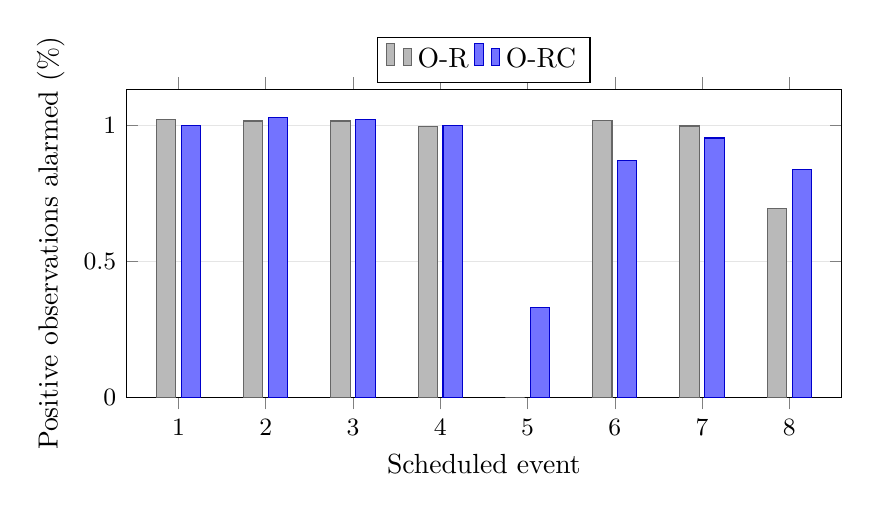
\begin{tikzpicture}
\begin{axis}[width=0.88\textwidth,height=5.5cm,ybar,bar width=7pt,xmin=0.4,xmax=8.6,ymin=0,xtick={1,...,8},xlabel={Scheduled event},ylabel={Positive observations alarmed (\%)},legend style={at={(0.5,1.02)},anchor=south,legend columns=2},ymajorgrids=true,grid style={gray!20},tick label style={font=\small}]
\addplot[fill=gray!55,draw=gray!80!black] coordinates {(1,1.023124465) (2,1.016203704) (3,1.016203704) (4,0.9953703704) (5,0) (6,1.018518519) (7,0.9976851852) (8,0.6944283697)};
\addplot[fill=blue!55,draw=blue!80!black] coordinates {(1,0.9999768524) (2,1.030092593) (3,1.020833333) (4,1) (5,0.3310185185) (6,0.8703703704) (7,0.9537037037) (8,0.8379435661)};
\legend{O-R,O-RC}
\end{axis}
\end{tikzpicture}

\caption{Fraction of positive observations alarmed within each event for the matched primary pair. Event 5 has no \method{O-R} alarm. Eight \method{O-RC} event hits coexist with sparse point coverage inside the long intervals.}\label{fig:eventcoverage}
\end{figure}

% claim: R09
\method{O-RC} first alarmed 9.20 seconds after the event-5 schedule flag. On the seven events both primary methods hit, five first-alarm delays were identical; \method{O-RC} was 2.05 seconds later on event 6 and approximately 0.05 seconds later on event 7. It was not earlier on any shared hit. Its detected-only median of 9.45 seconds, compared with 9.70 seconds for \method{O-R}, uses eight and seven events respectively and cannot establish faster matched detection.

% claim: R10
Each scheduled interval contains more than 43,000 positive observations. Any one alarm suffices for an overlap hit. \method{O-RC}'s eight hits therefore coexist with 342,559 false-negative positive observations, frequent normal episodes and AP near the prevalence reference. Short first-alarm delays here do not imply sustained recognition of the scheduled deviation or verified detection of its physical onset.

% claim: R11
\subsection{Measured resources}
Table~\ref{tab:resources} reports the whole-worker measurements. Both phases stayed within their frozen caps: scoring 900 seconds wall/600 seconds CPU and evaluation 1,800/1,200 seconds; both allowed 1 GiB worker resident memory and 256 MiB output. The hardware was a local Apple M5 Pro with 24 GiB host memory, using Python 3.15.0 and the standard library. No GPU or paid compute was used.

\begin{table}[htbp]\centering\small
\caption{Whole-phase resources, including source checks, parsing and output work. These are not isolated inference measurements.}\label{tab:resources}
\resizebox{\textwidth}{!}{\begin{tabular}{lrrrr}
\toprule
Phase & Wall (s) & CPU (s) & Peak RSS (MiB) & Output (MiB) \\
\midrule
score-final & 270.890 & 270.520 & 143.19 & 102.317 \\
evaluate-final & 44.778 & 44.660 & 902.50 & 0.188 \\
\bottomrule
\end{tabular}
}
\end{table}

% claim: R12
Per-method processing costs, initialization/parsing decomposition and per-record latency quantiles were not instrumented. The recorded whole-roster execution is locally feasible under its limits, but cannot determine whether the correction term's small gain had a measurable compute advantage or penalty relative to a control. No edge-device, transport-latency or live-deployment conclusion follows.

\section{Interpretation, limitations and independent evidence}
\label{sec:discussion}
% claim: L01
\subsection{What correction evidence contributed}
The narrow hypothesis receives limited descriptive support: at the frozen operating rule, adding the correction term increased F1 slightly and reduced normal alarm counts. It also added one event hit. That finding does not establish strong detection. The low positive-point recall and frequent normal episodes remain central, and ordinary controls offer comparable or stronger outcomes on several measures. The evidence does not warrant describing the method as a generally superior detector or a validated digital twin.

% claim: L02
The experiment cannot attribute the small gain to progression itself. Both primary outputs share nominal propagation, measurement correction and state history. Moreover, velocity measurements can retain direct speed evidence even after position is aligned: if $q(t)=q_0(\phi(t))$, then $\dot q(t)=q'_0(\phi(t))\dot\phi(t)$. Aligning $q$ need not remove the velocity-amplitude change. The similarity of direct-velocity and observer residual outcomes is consistent with that alternative explanation, but does not establish it causally. A different feature or alignment ablation prompted by this result would be a new exploratory analysis.

% claim: L03
The observer's uncertainty is also part of the interpretation. A mixture mean can poorly represent several plausible phases, as Equation~\eqref{eq:mixtureidentity} shows. The normal-development ambiguity and substantially better one-step autoregression suggest that the observer is not an especially accurate predictor for these inputs. A correction statistic might partly compensate for limitations of its residual representation. No independent phase truth, posterior-coverage calibration or causal mechanism experiment resolves that explanation here.

% claim: L04
\subsection{Limits of the evidence}
\paragraph{One acquisition.} The study contains one task recording with eight dependent intervention intervals. It supplies within-recording descriptions, not a sample of robots, factories, tasks or attack campaigns. We do not use an ordinary row bootstrap, treat intervals as independent deployments, or construct significance claims from deterministic repeated computation. No confidence interval is offered for a cross-robot population that was not sampled.

\paragraph{Ground truth and trust.} Schedule flags provide reproducible scoring boundaries but do not establish exact physical onset, malicious intent, trusted command provenance or healthy recovery. Truthful monitoring telemetry is an assumption. No result transfers to an adversary who consistently forges all monitored channels, nor establishes separation between faults, benign speed changes and attacks.

\paragraph{Development and model scope.} The same normal-development partition selected template resolution and supported observer diagnostics. That reuse is disclosed. The reference is an empirical collection of joint means, not a mechanically constrained model. Its inferred phase need not be unique, and the mean of possible states need not lie on a physically realizable trajectory. The free-running comparison is affected by numerical diffusion. Eleven methods do not constitute eleven independently reproduced recent papers or comprehensive detector benchmarking.

\paragraph{Operating rule and cost.} The normal-calibrated 99th percentile was fixed for the study; other alarm budgets, persistence rules and application utilities were not compared. We cannot infer an operationally acceptable false-alarm rate from this percentile. Per-method latency and computational overhead are unavailable. The scalar traces and current results cannot establish real-time transport, actuator safety or prevention of physical harm.

% claim: L05
\subsection{Planning fresh evidence after exposure}
The original final holdout is now exposed. A new score, threshold, persistence rule, input choice or preferred method motivated by these outcomes must be described as exploratory. Repeating or reshuffling the same recording does not create a new confirmation set. The local reproducibility package preserves the original outcome and separates future design decisions from it.

% claim: F01
Two public sources motivate a next admission audit rather than an immediate broader claim. The voraus-AD study provides separately collected robot executions with joint-state measurements and physical anomalies~\cite{voraus2024}. It could test whether a motion-only procedure applies to variable executions on another platform. It does not supply cyberattack intent. NIST's robot position-accuracy resource documents controller recordings under speed, payload and temperature conditions~\cite{nistdata}; these may support a benign-condition challenge after file and condition semantics are verified. Different condition files are not proof of recorded within-run changeovers. Neither source has been downloaded or admitted to this study.

% claim: F02
A future protocol must establish acquisition/session groups, original file identities, units, clock continuity and annotation provenance before fixing whole-group training, development, calibration and final assignments. CASPER's period, fitted scaler, 1,528-row warmup and gap rule cannot simply transfer. Source-specific refitting would test applicability, not zero-shot cross-robot transfer. Any newly developed model must be selected without new final outcomes; only a frozen model tested on genuinely reserved independent recordings could support a new confirmatory claim.

% claim: F03
A stronger cybersecurity question requires repeated acquisitions with documented authorized and unauthorized command changes, truthful monitoring, and trusted context that makes the distinction observable. Fault recordings alone cannot supply that evidence. No suitable laboratory access or independent cyber recording is assumed. The companion post-exposure evidence plan specifies admission gates, permitted claims and stopping decisions; it is a proposal, not an executed experiment or external preregistration.

\section{Conclusion}
% claim: C01
This controlled CASPER study found a small descriptive benefit from adding correction discrepancy to an empirical motion observer's residual: F1 increased from \RFone\ to \RCFone\ with slightly fewer normal alarms. Absolute detection remained weak. The correction variant alarmed on only \RCRecallPct\% of positive observations and produced \RCEpisodeRate\ normal episodes/hour, despite fresh alarms in all eight long scheduled intervals. Ordinary controls matched or exceeded several outcomes with different false-alarm costs.

Both primary variants retained nominal progression, so the comparison does not establish progression's isolated value. The evidence supports a narrow score-comparison finding and a caution about interpreting event hits without point coverage and normal burden. It establishes neither a novel digital twin nor general cybersecurity performance. Further design changes prompted by these exposed outcomes are exploratory; broader confirmation requires appropriately reserved independent recordings and a source-specific protocol.

\section*{Declarations and reproducibility}
% claim: A01
\paragraph{Data availability.}
The original CASPER provider and version are identified in Section~\ref{sec:data} and the data receipt~\cite{casperdata}. The provider metadata inspected at acquisition stated CC BY-SA 4.0. The original dataset is not redistributed in this manuscript package. A current provider download must be matched to the recorded file size and SHA-256; a similarly named or newer release must not be silently substituted. The package includes aggregate results, source identities and an access recipe, not private download information or raw trajectories. Redistribution terms for data-derived artifacts require review before public release.

% claim: A02
\paragraph{Code and artifact availability.}
A local draft package contains the exact 52 tested source/configuration files, historical scientific specifications, frozen aggregate results, a deterministic table/figure generator, the bibliography and verification scripts. No upstream vendor code or third-party paper figures are bundled. Saved row-level scores, fitted models, complete run snapshots, resource logs and original access ledgers remain in local experiment storage, with identities recorded in the package. The public repository/archive, release identifier and code license are \pending{not selected or approved}. Regenerating presentation assets is not an independent rerun of data loading, fitting and scoring. The reproduction guide explicitly separates these levels.

% claim: A03
\paragraph{Author contributions.}
The requested author order is Muhammad Usman, then Haiqa Mushtaq. Individual conceptualization, methodology, software, validation, formal analysis, data curation and writing roles are \pending{each author's actual Contributor Roles Taxonomy (CRediT) contributions}. Project-folder ownership and assistant work do not establish human contributions. Affiliations, corresponding author and approval of the manuscript by both authors are \pending{confirmation}.

\paragraph{Funding and competing interests.}
Funding sources, grant identifiers and competing interests are \pending{author declarations}. The absence of an entry is not a declaration of no funding or no conflicts.

% claim: A04
\paragraph{Ethics and permissions.}
This work analyzes an existing robot dataset; no new human-participant recruitment or physical robot intervention was conducted by this study. No institutional exemption or ethics approval is claimed. Any applicable institutional determination remains \pending{author/institution confirmation}. Manuscript tables and plots are newly generated from our saved aggregate outputs, with no copied third-party figures. The local package has not been published or submitted. Dataset terms, code licensing and any source-specific obligations must be checked before distribution; access to a paper does not automatically permit republishing its content.

% claim: A05
\paragraph{AI-assistance disclosure.}
Artificial intelligence (AI) assistance through OpenAI Codex was used for research planning, primary-source checks, software implementation and tests, experiment orchestration, result analysis, manuscript drafting and reproducibility checks. The reported numerical findings come from preserved executable runs, not generated hypothetical benchmark results. Human reading, interpretation and approval of all claims and code remain to be confirmed by the authors; this draft does not attest that those checks have happened. Tool/version records available in the work logs should accompany the eventual disclosure. Exact model identifiers for sessions not recorded are not inferred. No target journal has been selected, so venue-specific AI-use requirements remain unresolved and must be checked against that venue's current policy before submission.

\clearpage
\appendix
\section{Exact identity and completed execution}
\label{app:identity}
% claim: P01
All row ranges are zero-based data-row indices excluding the header. The original right-arm SHA-256 is
\begin{quote}\small\path{181662e25de09c1f4ed05e0877a65c40225752d6f54575ddb1cdf8a0cf29a334}.\end{quote}
The selection freeze is
\begin{quote}\small\path{3b3f62ad323fec96aa5940ea081b668286829064a90225293e4790256baa3b36},\end{quote}
and the immutable pre-execution final freeze is
\begin{quote}\small\path{1fd7767bdcd4e5203de7180f9e78cb6d82e35c2d7e2b5564821634fedf295a1d}.\end{quote}
The latter retains historical not-started fields; actual completion is in the separate completion record. Experiment code was recorded at Git revision \path{b207e0758c1dd90fbd09d3aa4de943a11d7f08cb} with dirty-worktree patches and exact file snapshots. That revision alone is insufficient to reconstruct the executed bytes. The package binds the full tested file inventory instead of treating the manuscript's later repository revision as the experimental version.

% claim: P02
The protected scoring run began at 06:21:17.705600 UTC on 17 October 2026 and was accepted at 06:25:51.061961 UTC. Label joining began at 06:26:30.415287 UTC, after all streams sealed; evaluation completed at 06:27:12.073582 UTC. The source checksum matched before and after both phases. Logical access and attempt records provide procedural protection, not an operating-system lock or an independent data custodian. Historical completed commands, from the manufacturing project directory, are:
\begin{verbatim}
.venv/bin/python scripts/run_campaign.py --check-final
.venv/bin/python scripts/run_campaign.py --score-final
.venv/bin/python scripts/run_campaign.py --evaluate-final \
  --score-run experiments/runs/\
campaign_v0.1_score-final_2026-10-17T062117.703085_0000
\end{verbatim}
These commands document consumed attempts. They are not instructions to remove ledgers or rerun the exposed campaign in place. The reproduction guide specifies fresh-workspace and artifact requirements separately.

\section{Candidate selection and frozen thresholds}
\label{app:selection}
% claim: P03
Table~\ref{tab:selection} retains every declared ordinary candidate. Template and autoregression objectives are mean standardized prediction MSE; the velocity score is a different quantity and is not a cross-family objective. Its singleton is retained without selection. Exact ties follow the declared order. The observer's fixed mixing rate, training-only bandwidth and mean scales are specified in Section~\ref{sec:methods}. There were no neural checkpoints or attack-selected seeds.
\begin{table}[htbp]\centering\small
\caption{All normal-development candidate outcomes; differently defined family scores must not be ranked together.}\label{tab:selection}
\begin{tabular}{lrr}
\toprule
Candidate & Development objective & Selected \\
\midrule
velocity\_zmax & 0.851959918 & yes \\
template\_bins32 & 0.374222865 & yes \\
template\_bins64 & 0.417253723 & no \\
ar\_p1\_ridge0.001 & 0.006315019 & no \\
ar\_p1\_ridge0.1 & 0.014515634 & no \\
ar\_p4\_ridge0.001 & 0.002093570 & yes \\
ar\_p4\_ridge0.1 & 0.017794516 & no \\
\bottomrule
\end{tabular}

\end{table}
\begin{table}[htbp]\centering\small
\caption{Thresholds fixed by the same rank rule. Digits reflect stored binary64 values, not physical measurement precision.}\label{tab:thresholds}
\begin{tabular}{lr}
\toprule
Method & Frozen threshold \\
\midrule
O-R & 13.985559778490424 \\
O-RC & 16.463814217165016 \\
O-C & 0.015377372026598208 \\
O-K & 0.056350365425031253 \\
O-L & 7.2153891565675412 \\
O-Rv & 9.3021804164182704 \\
O-Follow & 14.839281942008819 \\
O-Free & 23.009252694772172 \\
V-Z & 6.5701205181677951 \\
T-32 & 4.9056682511855545 \\
AR-4 & 0.036774935278963361 \\
\bottomrule
\end{tabular}

\end{table}

\section{Complete counts, event delays and recovery intervals}
\label{app:events}
% claim: P04
Table~\ref{tab:counts} preserves all confusion counts and protected-normal alarm counts. Mixed counts use 682,646 observations; normal point counts use 214,473 eligible observations. All normal boundary-censoring counts were zero in this campaign. All eight event intervals were fully eligible. Their half-open rows are $[1080004,1123205)$, $[1166405,1209605)$, $[1252805,1296005)$, $[1339205,1382405)$, $[1425606,1468806)$, $[1512006,1555206)$, $[1598406,1641606)$ and $[1684806,1728007)$.

\begin{table}[htbp]\centering\small
\caption{Mixed confusion counts and separate protected-normal burden.}\label{tab:counts}
\resizebox{\textwidth}{!}{\begin{tabular}{lrrrrrr}
\toprule
Method & TP & FP & FN & TN & Normal alarms & Episodes \\
\midrule
O-R & 2,921 & 3,349 & 342,681 & 333,695 & 2,159 & 564 \\
O-RC & 3,043 & 3,317 & 342,559 & 333,727 & 2,132 & 554 \\
O-C & 3,354 & 3,233 & 342,248 & 333,811 & 2,115 & 1,021 \\
O-K & 3,379 & 3,301 & 342,223 & 333,743 & 2,127 & 1,041 \\
O-L & 2,942 & 3,373 & 342,660 & 333,671 & 2,156 & 564 \\
O-Rv & 2,919 & 3,352 & 342,683 & 333,692 & 2,155 & 564 \\
O-Follow & 2,892 & 3,320 & 342,710 & 333,724 & 2,154 & 564 \\
O-Free & 2,924 & 3,345 & 342,678 & 333,699 & 2,137 & 564 \\
V-Z & 2,908 & 3,383 & 342,694 & 333,661 & 2,138 & 564 \\
T-32 & 13,899 & 12,441 & 331,703 & 324,603 & 3,002 & 597 \\
AR-4 & 3,319 & 3,311 & 342,283 & 333,733 & 2,109 & 1,302 \\
\bottomrule
\end{tabular}
}
\end{table}
\begin{table}[htbp]\centering\scriptsize
\caption{All schedule-relative delays in seconds. Each observed overlap was also a fresh onset here; MISS remains undefined, not zero. Native-time values are rounded only for presentation.}\label{tab:delays}
\resizebox{\textwidth}{!}{\begin{tabular}{lrrrrrrrrr}
\toprule
Method & E1 & E2 & E3 & E4 & E5 & E6 & E7 & E8 & Misses \\
\midrule
O-R & 9.70 & 3.45 & 10.10 & 8.85 & MISS & 4.60 & 29.00 & 12.05 & 1 \\
O-RC & 9.70 & 3.45 & 10.10 & 8.85 & 9.20 & 6.65 & 29.05 & 12.05 & 0 \\
O-C & 9.25 & 3.00 & 9.65 & 8.40 & 6.25 & 4.15 & 1.85 & 9.45 & 0 \\
O-K & 9.25 & 3.00 & 9.65 & 8.40 & 6.25 & 4.10 & 1.85 & 9.45 & 0 \\
O-L & 9.70 & 3.45 & 10.10 & 8.85 & MISS & 4.60 & 29.00 & 12.05 & 1 \\
O-Rv & 9.70 & 3.45 & 10.10 & 8.85 & MISS & 4.60 & 29.00 & 12.05 & 1 \\
O-Follow & 9.70 & 3.45 & 10.10 & 8.85 & MISS & 4.55 & 29.00 & 12.10 & 1 \\
O-Free & 9.70 & 3.45 & 10.10 & 8.85 & MISS & 4.60 & 29.00 & 12.10 & 1 \\
V-Z & 9.70 & 3.40 & 10.10 & 8.85 & MISS & 4.55 & 29.00 & 12.10 & 1 \\
T-32 & 9.65 & 3.30 & 9.95 & 8.60 & 9.05 & 4.40 & 28.85 & 9.75 & 0 \\
AR-4 & 9.80 & 3.55 & 10.20 & 8.95 & 8.80 & 4.70 & 28.35 & 11.70 & 0 \\
\bottomrule
\end{tabular}
}
\end{table}

% claim: P05
Table~\ref{tab:recovery} reports all eight scheduled-zero intervals following successive events. Columns Z1--Z7 end at the next event start; Z8 ends at the recording's end. Entries are alarm observations divided by eligible observations. These intervals are not independently certified recovery states. Full start/end rows, native exposure, episode rates and censoring are retained in the aggregate JSON, so the table does not replace the detailed record.
\begin{table}[htbp]\centering\scriptsize
\caption{All scheduled-zero intervals: alarm points / eligible points.}\label{tab:recovery}
\resizebox{\textwidth}{!}{\begin{tabular}{lrrrrrrrr}
\toprule
Method & Z1 & Z2 & Z3 & Z4 & Z5 & Z6 & Z7 & Z8 \\
\midrule
O-R & 419/43200 & 437/43200 & 426/43200 & 432/43201 & 427/43200 & 435/43200 & 434/43200 & 339/34643 \\
O-RC & 421/43200 & 432/43200 & 427/43200 & 422/43201 & 422/43200 & 430/43200 & 423/43200 & 340/34643 \\
O-C & 418/43200 & 425/43200 & 422/43200 & 423/43201 & 401/43200 & 408/43200 & 408/43200 & 328/34643 \\
O-K & 429/43200 & 429/43200 & 425/43200 & 435/43201 & 408/43200 & 417/43200 & 420/43200 & 338/34643 \\
O-L & 422/43200 & 435/43200 & 427/43200 & 430/43201 & 433/43200 & 440/43200 & 440/43200 & 346/34643 \\
O-Rv & 419/43200 & 435/43200 & 427/43200 & 433/43201 & 427/43200 & 436/43200 & 434/43200 & 341/34643 \\
O-Follow & 417/43200 & 428/43200 & 426/43200 & 428/43201 & 425/43200 & 425/43200 & 430/43200 & 341/34643 \\
O-Free & 424/43200 & 433/43200 & 429/43200 & 425/43201 & 428/43200 & 436/43200 & 432/43200 & 338/34643 \\
V-Z & 425/43200 & 435/43200 & 442/43200 & 438/43201 & 425/43200 & 432/43200 & 437/43200 & 349/34643 \\
T-32 & 1314/43200 & 1329/43200 & 2018/43200 & 1302/43201 & 1363/43200 & 1296/43200 & 2419/43200 & 1400/34643 \\
AR-4 & 418/43200 & 418/43200 & 435/43200 & 426/43201 & 430/43200 & 428/43200 & 423/43200 & 333/34643 \\
\bottomrule
\end{tabular}
}
\end{table}

\section{Artifact regeneration and claim traceability}
\label{app:package}
% claim: P06
The manuscript package's \path{editorial/CLAIM_EVIDENCE_MAP.json} maps named claim groups to primary-source locations or exact experiment/configuration records. \path{editorial/references.json} records source versions and access limits; \path{references.bib} and the DOI-visible bibliography are generated from that register. \path{generated/ASSET_MANIFEST.json} binds every generated table, numerical macro and PGFPlots figure to the saved inputs and generator. No figure uses raw trajectories or newly tuned outputs. The verifier checks source identities, citation keys, cross-references, complete method/event coverage and deterministic regeneration. These checks do not substitute for author comprehension, external peer review or visual PDF inspection.

\clearpage
\begin{thebibliography}{99}

\bibitem{casper2024} Hakan Kayan, Ryan Heartfield, Omer Rana, Pete Burnap, Charith Perera. CASPER: Context-Aware IoT Anomaly Detection System for Industrial Robotic Arms. \emph{ACM Transactions on Internet of Things}, 5(3), Article 18, 36 pages, 2024. DOI: \href{https://doi.org/10.1145/3670414}{\nolinkurl{10.1145/3670414}}. \url{https://iotgarage.net/publications/pdfs/Kayan2024a.pdf}. Corrected version of record V1.1, 5 February 2025; original publication August 2024.

\bibitem{casperdata} Hakan Kayan. Industrial Robotic Arm -- Pick and Place Dataset. \emph{Kaggle, original collection, version 3}, 2023. \url{https://www.kaggle.com/datasets/hkayan/industrial-robotic-arm-anomaly-detection}. Provider version 3, 11 February 2023; received 16 October 2026.

\bibitem{edge2025} Hakan Kayan, Ryan Heartfield, Omer Rana, Pete Burnap, Charith Perera. Real-Time Anomaly Detection for Industrial Robotic Arms Using Edge Computing. \emph{IEEE Internet of Things Journal}, 12(15), 29696--29712, 2025. DOI: \href{https://doi.org/10.1109/JIOT.2025.3569780}{\nolinkurl{10.1109/JIOT.2025.3569780}}. \url{https://iotgarage.net/publications/pdfs/Kayan2025a.pdf}. Author manuscript; publisher issue 1 August 2025; first-online day unverified.

\bibitem{twine2026} Mubashar Iqbal, Sabah Suhail, Simon Freudenthaler, Muhammad Fahim, Raimundas Matulevičius. TWINE: ISO 23247-compliant digital twin and explainable AI framework for anomaly detection. \emph{Internet of Things}, 38, 101976, 2026. DOI: \href{https://doi.org/10.1016/j.iot.2026.101976}{\nolinkurl{10.1016/j.iot.2026.101976}}. \url{https://pureadmin.qub.ac.uk/ws/files/689658736/TWINE.pdf}. QUB accepted manuscript; journal issue July 2026.

\bibitem{willsky1976} Alan S. Willsky. A Survey of Design Methods for Failure Detection in Dynamic Systems. \emph{Automatica}, 12(6), 601--611, 1976. DOI: \href{https://doi.org/10.1016/0005-1098(76)90041-8}{\nolinkurl{10.1016/0005-1098(76)90041-8}}. \url{https://willsky.lids.mit.edu/publ_pdfs/15_pub_AUTO.pdf}. Published survey; foundational background outside recent-baseline window.

\bibitem{campbell2017} Joseph Campbell, Heni Ben Amor. Bayesian Interaction Primitives: A SLAM Approach to Human-Robot Interaction. \emph{Proceedings of the 1st Annual Conference on Robot Learning, PMLR}, 78, 379--387, 2017. \url{https://proceedings.mlr.press/v78/campbell17a.html}. PMLR conference version; DOI not verified.

\bibitem{clark2020} Geoffrey Clark, Joseph Campbell, Seyed Mostafa Rezayat Sorkhabadi, Wenlong Zhang, Heni Ben Amor. Predictive Modeling of Periodic Behavior for Human-Robot Symbiotic Walking. \emph{IEEE International Conference on Robotics and Automation}, 7599--7605, 2020. DOI: \href{https://doi.org/10.1109/ICRA40945.2020.9196676}{\nolinkurl{10.1109/ICRA40945.2020.9196676}}. \url{https://arxiv.org/abs/2005.13139v1}. ICRA metadata; method inspected in author preprint v1, 27 May 2020.

\bibitem{park2016} Daehyung Park, Zackory Erickson, Tapomayukh Bhattacharjee, Charles C. Kemp. Multimodal Execution Monitoring for Anomaly Detection During Robot Manipulation. \emph{IEEE International Conference on Robotics and Automation}, 407--414, 2016. DOI: \href{https://doi.org/10.1109/ICRA.2016.7487160}{\nolinkurl{10.1109/ICRA.2016.7487160}}. \url{https://pidipidi.github.io/pdf/ICRA16_2378_FI.pdf}. Author manuscript for ICRA 2016; foundational background.

\bibitem{itti2005} Laurent Itti, Pierre F. Baldi. Bayesian Surprise Attracts Human Attention. \emph{Advances in Neural Information Processing Systems}, 18, 2005. \url{https://papers.neurips.cc/paper_files/paper/2005/hash/0172d289da48c48de8c5ebf3de9f7ee1-Abstract.html}. Official NIPS 2005 conference record; author 2006 proceedings citation is not mixed into this entry; DOI not verified.

\bibitem{xu2022} Jiehui Xu, Haixu Wu, Jianmin Wang, Mingsheng Long. Anomaly Transformer: Time Series Anomaly Detection with Association Discrepancy. \emph{arXiv:2110.02642v5}, 2022. DOI: \href{https://doi.org/10.48550/arXiv.2110.02642}{\nolinkurl{10.48550/arXiv.2110.02642}}. \url{https://arxiv.org/abs/2110.02642v5}. Author manuscript v5, 29 June 2022; ICLR-related work, citation explicitly identifies inspected arXiv version.

\bibitem{arp2022} Daniel Arp, Erwin Quiring, Feargus Pendlebury, Alexander Warnecke, Fabio Pierazzi, Christian Wressnegger, Lorenzo Cavallaro, Konrad Rieck. Dos and Don'ts of Machine Learning in Computer Security. \emph{31st USENIX Security Symposium}, 3971--3988, 2022. \url{https://www.usenix.org/conference/usenixsecurity22/presentation/arp}. Official 2022 proceedings; DOI not verified.

\bibitem{voraus2024} Jan Thieß Brockmann, Marco Rudolph, Bodo Rosenhahn, Bastian Wandt. The voraus-AD Dataset for Anomaly Detection in Robot Applications. \emph{IEEE Transactions on Robotics}, 40, 438--451, 2024. DOI: \href{https://doi.org/10.1109/TRO.2023.3332224}{\nolinkurl{10.1109/TRO.2023.3332224}}. \url{https://arxiv.org/abs/2311.04765}. Journal volume 2024, institution reports online 13 November 2023; author preprint v1 inspected.

\bibitem{nistdata} National Institute of Standards and Technology. Degradation Measurement of Robot Arm Position Accuracy. \emph{NIST data resource}. DOI: \href{https://doi.org/10.18434/M31962}{\nolinkurl{10.18434/M31962}}. \url{https://www.nist.gov/el/intelligent-systems-division-73500/degradation-measurement-robot-arm-position-accuracy}. Provider page accessed 17 October 2026; page/catalogue dates are not claimed as acquisition dates.

\end{thebibliography}

\end{document}
